\chapter{Anwendung der Pulsoxymetrie}
\begin{itemize}
    \item Das Gerät wird eingeschaltet und auf einen Finger geclipt
    \item Zeigt dann Puls und Sauerstoffsättigung an
    \item Messungenauigkeiten können z.B. durch Nagellack, Handcreme, schlechter Durchblutung der Finger entstehen
          \begin{itemize}
              \item Nagellack $\implies$ Gerät kann auch seitlich angebracht werden
          \end{itemize}
\end{itemize}
\section*{Pulswerte}
\begin{figure}[H]
    \centering
    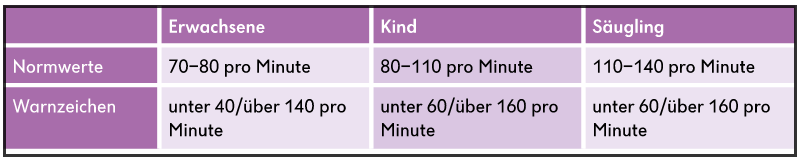
\includegraphics[width=\textwidth]{res/puls.png}
\end{figure}